\documentclass[]{article}

%opening
\title{}
\author{}
\usepackage{indentfirst}
\usepackage{graphicx}
\begin{document}

\maketitle

\begin{table}[htb]\renewcommand{\arraystretch}{1.4}
	\centering
	\caption{Notations}
	\label{notations}
	\begin{tabular}{c c l}
		\hline
		Notations           & Unit                & \multicolumn{1}{c}{Description}              \\ \hline
		 $x_{ij}^{*}$  & \ & The normalization data \\
		 $\overline{x_{j}}$ &\ & The mean of the column\\
		 $\sigma_{j}$ &\ &The standard deviation of the column\\
		 $y$  &\ & Total energy consumption\\
		 $k_{i}$  &\ &Regression coefficient\\
		 $\beta_{0}$  &\ & Regression intercept\\ \hline
	\end{tabular}
\end{table}

\section{Model }
\subsection{Description of the model}


We build a multiple regression model to help analysis the data.


The selection of regression variables has practical significance.  In order to make the model easy to do structural analysis,  control and forecast,  it is the best way to select the best variable from the subsets of the original variables.  The original data contains 605 variables,  there is no doubt that filtrating some important variables is the first step.  We choose principal component analysis(PCA) to decrease the variable because it reduce the compution complexity.\textbf{citation pca}


After data normalization,  the regression coefficient can be regarded as the importance of the corresponding variable.  We choose every five years' data as a dataset to estimate a regression line.  Then we get 46 sets  of  regression coefficient which can reflect the evolvement of the energy profile.  The equation of the regression is:
\begin{equation}
y = k_{1}x_{1}+ k_{2}x_{2}+...+k_{n}x_{n}+\beta_{0}
\end{equation}
$y$  is total energy consumption, $k_{i}$  is regression coefficient and $\beta_{0}$  is regression intercept.
\subsection{Normalize The Data}
The orginal data contains various different variables and the variables have different dimensions.  Before excute principal component analysis, the first step is to normalize the data.  
\begin{equation}
    x_{ij}^{*} = \frac{x_{ij}-\overline{x_{j}}}{\sigma_{j}}  
\end{equation}
$x_{ij}^{*} $  is the normalization data.  $\overline{x_{j}}$  is the mean of the column and $\sigma_{j}$  is the standard deviation of the column.  We use python to process the data, the code is included in the appendix.
\subsection{The Result of  PCA And Mutiple Regression}


We use R language to excute PCA and python to excute multiple regerssion. The code is included in the apendix.
\subsubsection{Arizona}
	\begin{table}[h]\renewcommand{\arraystretch}{1.4}
	\newcommand{\tabincell}[2]{\begin{tabular}{@{}#1@{}}#2\end{tabular}}
		\centering
		\caption{Main variables of Arizona}
		\label{notations}
		\begin{tabular}{l l}
			\hline
			MSN               & Description              \\ \hline
		CLTCV	& Coal total expenditures.\\ 
		CLCCV	&Coal expenditures in the commercial sector.\\
		CLACB	&Coal consumed by the transportation sector.\\
		ESCCV	&Electricity expenditures in the commercial sector.\\
		ESRCV	&Electricity expenditures in the residential sector.\\
		ESTCB	&Electricity total consumption (i.e., sold).\\
		
		ESTCV	&Electricity total expenditures.\\
		
		GECCB	&\tabincell{l}{Direct use of geothermal energy and heat\\ pumps in the commercial sector.}\\
		NGACB	&Natural gas consumed by the transportation sector. \\
		NGCCV	&\tabincell{l}{Natural gas expenditures in the commercial sector\\ (including supplemental gaseous fuels).}\\
		NGTCV&\tabincell{l}{Natural gas total expenditures\\ (including supplemental gaseous fuels).}\\
		NNCCB	&\tabincell{l}{Natural gas consumed by (delivered to) the commercial sector\\ (excluding supplemental gaseous fuels).  (Code used in SEDS 2006.)}\\
		PAACV	&\tabincell{l}{All petroleum products total expenditures \\in the transportation sector.}\\
		SOEGB	&\tabincell{l}{Electricity produced from photovoltaic and \\solar thermal energy by the electric power sector.}\\
		 \hline
		\end{tabular}
	\end{table}
\begin{figure}[htb]
	\caption{The  energy profile evolvement of Arizona}
	\label{fig:Arizona energy profile}
	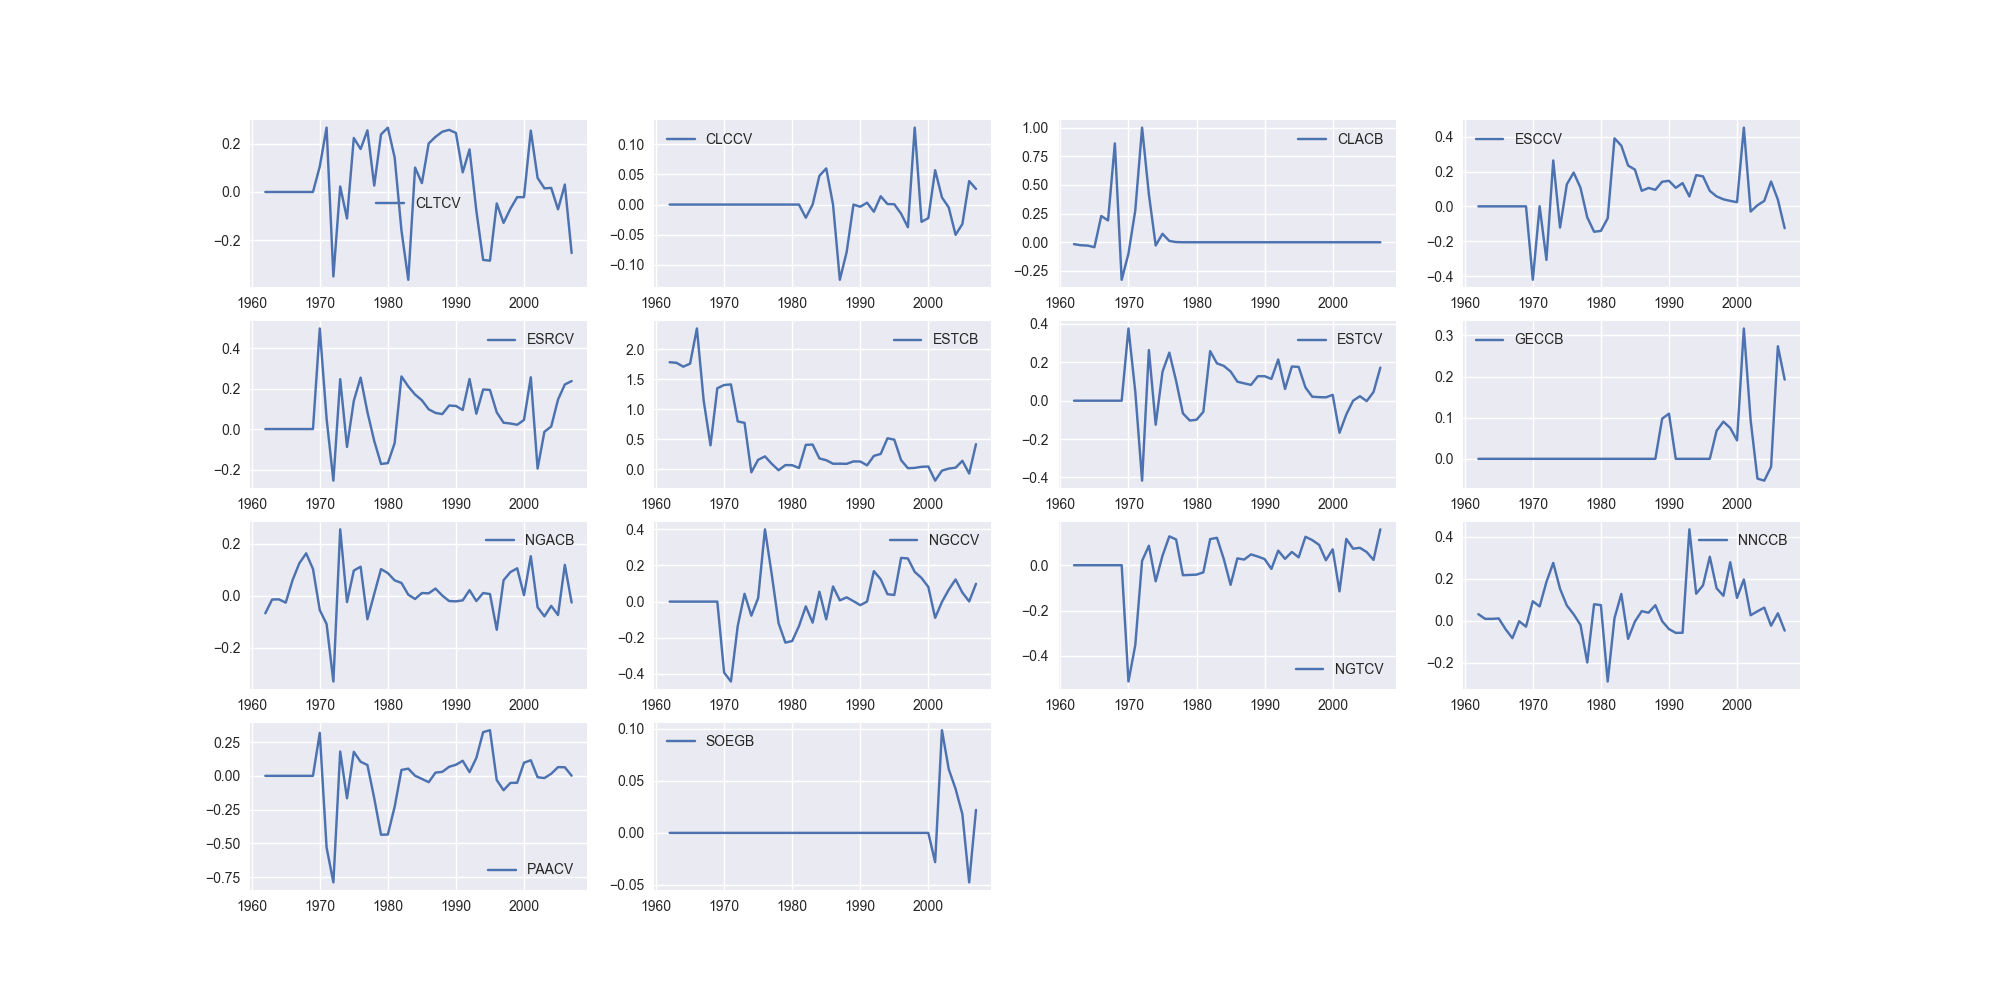
\includegraphics[scale=0.3]{az.png}
\end{figure}
\subsubsection{California}
\begin{table}[h]\renewcommand{\arraystretch}{1.4}
	\newcommand{\tabincell}[2]{\begin{tabular}{@{}#1@{}}#2\end{tabular}}
	\centering
	\caption{Main variables of California}
	\label{notations}
	\begin{tabular}{l l}
		\hline
		MSN               & Description              \\ \hline
     BMTCB	&Biomass total consumption\\
     CLCCB	&Coal consumed by the commercial sector.\\
     CLEIB	&Coal consumed by the electric power sector.\\
     CLICV	&Coal expenditures in the industrial sector.\\
     ELIMB	&Electricity imported into the United States.\\
     ESCCV	&Electricity expenditures in the commercial sector.\\
     ESICB	&Electricity consumed by (i.e., sold to) the industrial sector.\\
     ESTCB	&Electricity total consumption (i.e., sold).\\
     NGCCV	&\tabincell{l}{Natural gas expenditures in the commercial sector\\ (including supplemental gaseous fuels).}\\
     NGRCV	&\tabincell{l}{Natural gas expenditures in the residential sector\\(including supplemental gaseous fuels).}\\
     NNCCB	&\tabincell{l}{Natural gas consumed by (delivered to) the commercial sector \\(excluding supplemental gaseous fuels).  (Code used in SEDS 2006.)}\\
     PAACV	&All petroleum products total expenditures in the transportation sector.\\
     NUETB	&Electricity produced from nuclear power.\\
  
     \hline
\end{tabular}
\end{table}
\begin{figure}[h]
	\caption{The  energy profile evolvement of California}
	\label{fig:California energy profile}
	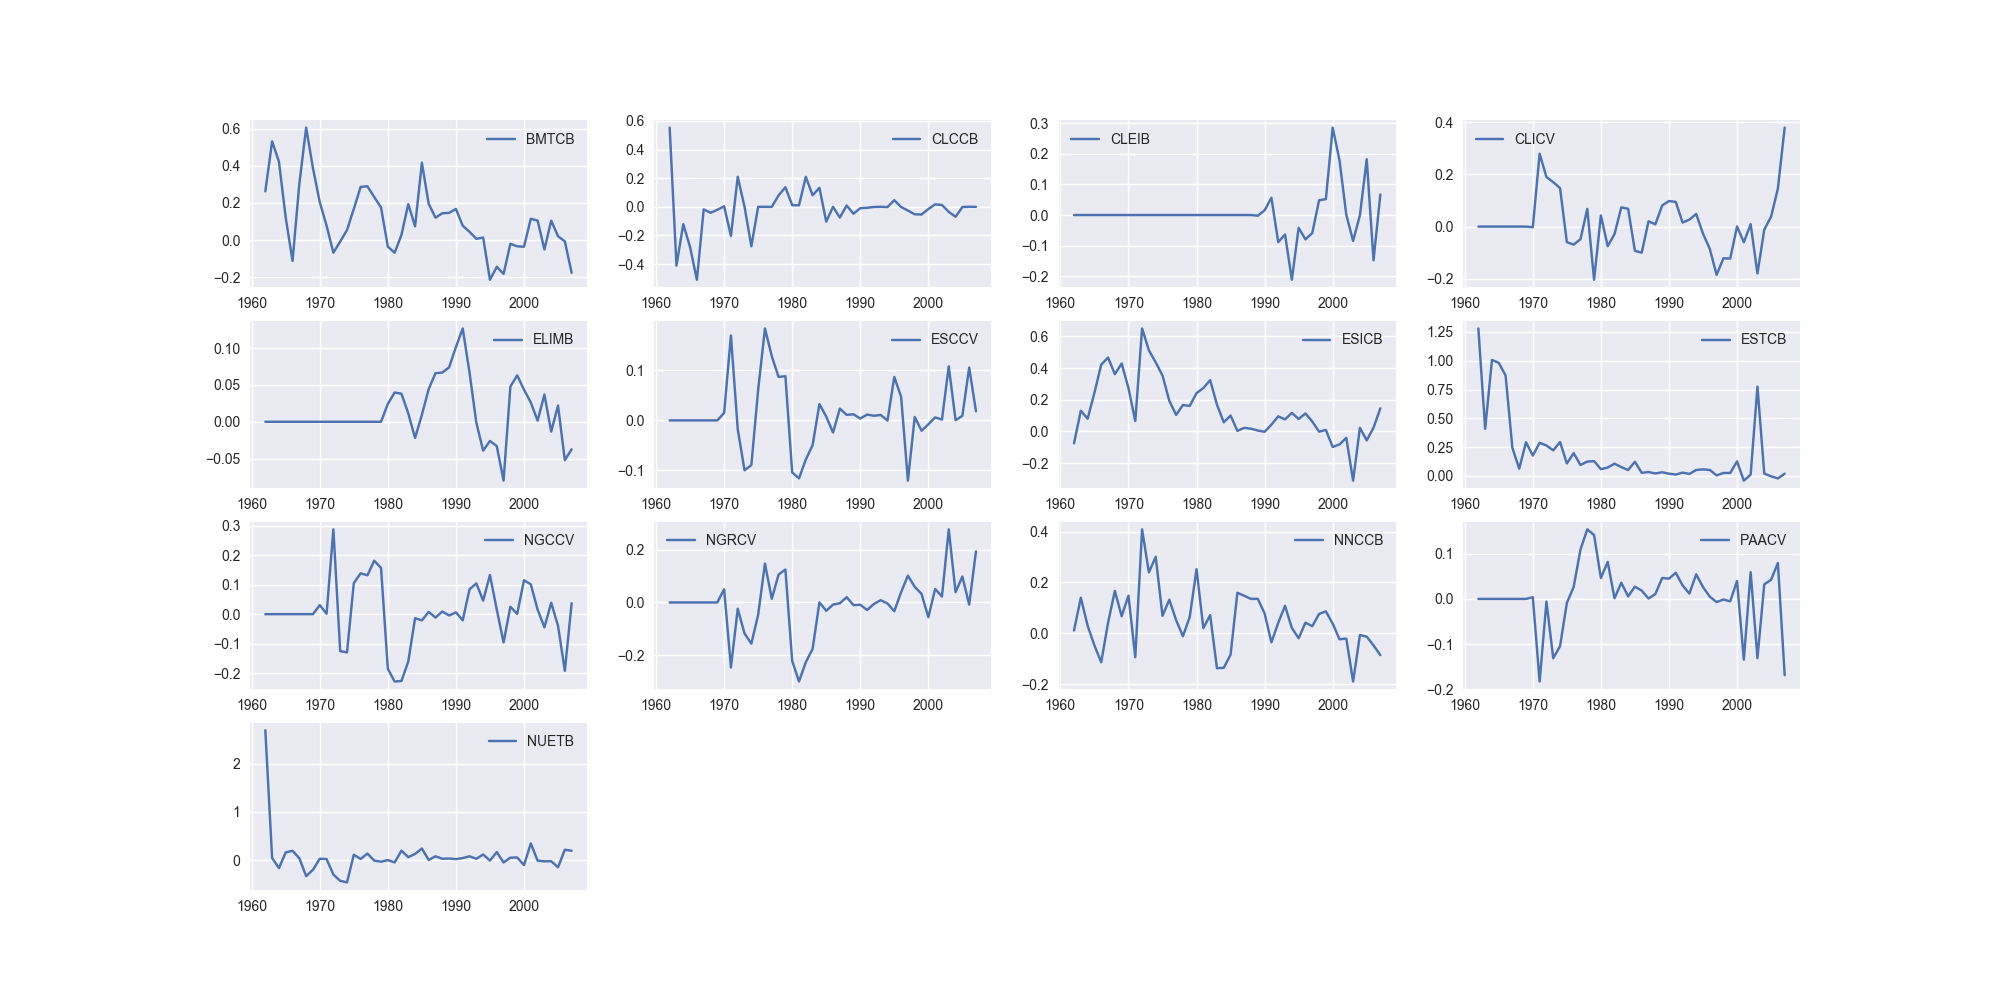
\includegraphics[scale=0.3]{ca.png}
\end{figure}
\subsubsection{New Mexico}
\begin{table}[h]\renewcommand{\arraystretch}{1.4}
	\newcommand{\tabincell}[2]{\begin{tabular}{@{}#1@{}}#2\end{tabular}}
	\centering
	\caption{Main variables of New Mexico}
	\label{notations}
	\begin{tabular}{l l}
		\hline
		MSN               & Description              \\ \hline
CLPRB	&Coal production.\\
	CLTCV	&Coal total expenditures.\\
CLCCB	&Coal consumed by the commercial sector.\\
 CLICV	&Coal expenditures in the industrial sector.\\
 ESCCB	&Electricity consumed by (i.e., sold to) the commercial sector.\\
 ESICB	&Electricity consumed by (i.e., sold to) the industrial sector.\\
GETCB	&Geothermal energy total consumption.\\

 GEICB	&Direct use of geothermal energy and heat pumps in the industrial sector.\\
 LOTCB	&Total electrical system energy losses.\\
 
 NGACB	&Natural gas consumed by the transportation sector. \\
 NGCCV	&\tabincell{l}{Natural gas expenditures in the commercial sector \\(including supplemental gaseous fuels).}\\
 NGICV	&\tabincell{l}{Natural gas expenditures in the industrial sector \\(including supplemental gaseous fuels).}\\
 NGTCB	&Natural gas total consumption (including supplemental gaseous fuels).\\
 
\hline
\end{tabular}
\end{table}
\begin{figure}[htb]
	\caption{The  energy profile evolvement of New Mexico}
	\label{fig:New Mexico energy profile}
	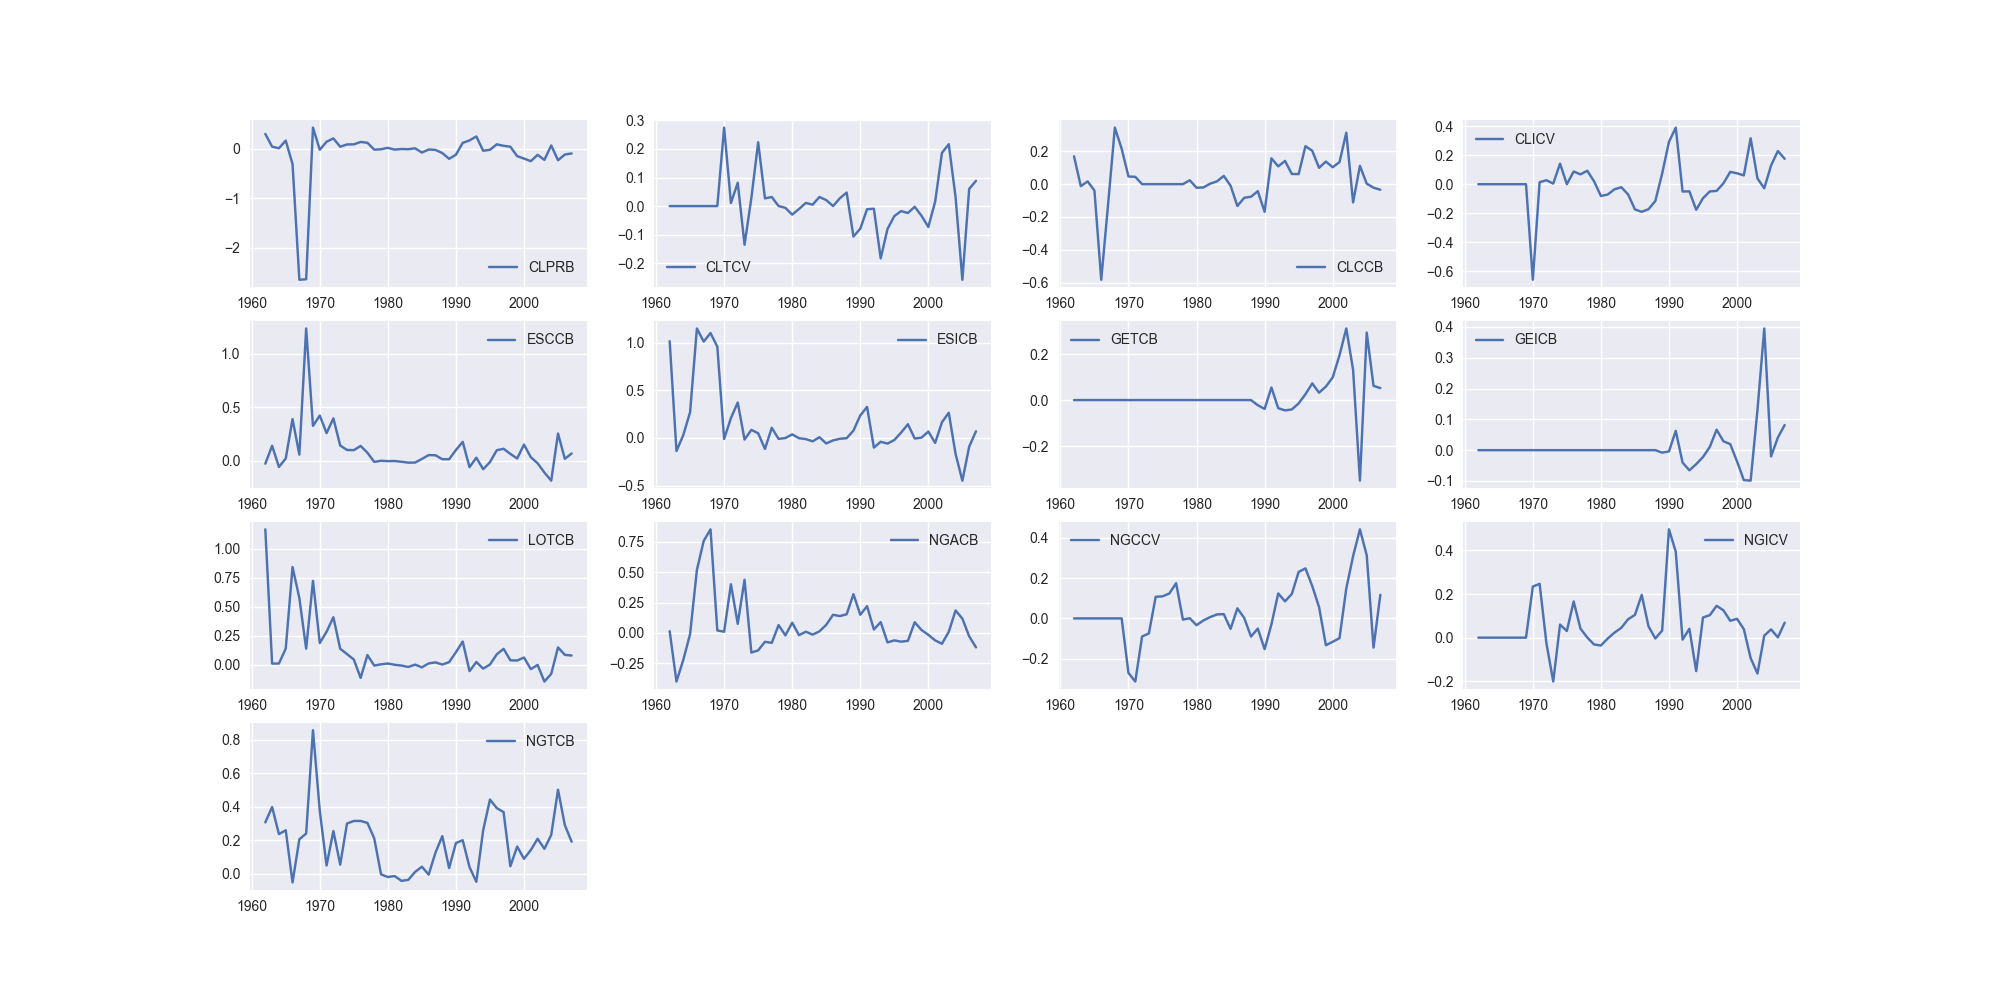
\includegraphics[scale=0.3]{nm.png}
\end{figure}

\subsubsection{Texas}
\begin{table}[h]\renewcommand{\arraystretch}{1.4}
	\newcommand{\tabincell}[2]{\begin{tabular}{@{}#1@{}}#2\end{tabular}}
	\centering
	\caption{Main variables of Texas}
	\label{notations}
	\begin{tabular}{l l}
		\hline
		MSN               & Description              \\ \hline
		CLCCB	&Coal consumed by the commercial sector.\\
		CLACB	&Coal consumed by the transportation sector.\\
		CLRCB	&Coal consumed by the residential sector.\\
		ELIMV	&Electricity imports expenditures.\\
		ESRCV	&Electricity expenditures in the residential sector.\\
		ESTCV	&Electricity total expenditures.\\
		GDPRV	&Current-dollar gross domestic product.\\
		GETCB	&Geothermal energy total consumption.\\
		HYICB	&Hydroelectricity produced in the industrial sector.\\
		HYTCB	&Hydroelectricity total production.\\
		
		NGCCB	&\tabincell{l}{Natural gas consumed by (delivered to) the commercial sector \\(including supplemental gaseous fuels).}\\
		NGCCV	&\tabincell{l}{Natural gas expenditures in the commercial sector \\(including supplemental gaseous fuels).}\\
		NGRCB	&\tabincell{l}{Natural gas consumed by (delivered to) the residential sector\\ (including supplemental gaseous fuels).}\\
		NGTCV	&Natural gas total expenditures (including supplemental gaseous fuels).\\
		NNACB	&Natural gas consumed by the transportation sector.  (Code used in SEDS 2006.)\\
		PACCV	&All petroleum products total expenditures in the commercial sector.\\
		WYTCB	&Electricity produced from wind energy.\\
		
		\hline
	\end{tabular}
\end{table}
\begin{figure}[htb]
\caption{The  energy profile evolvement of Texas}
\label{fig:Texas energy profile}
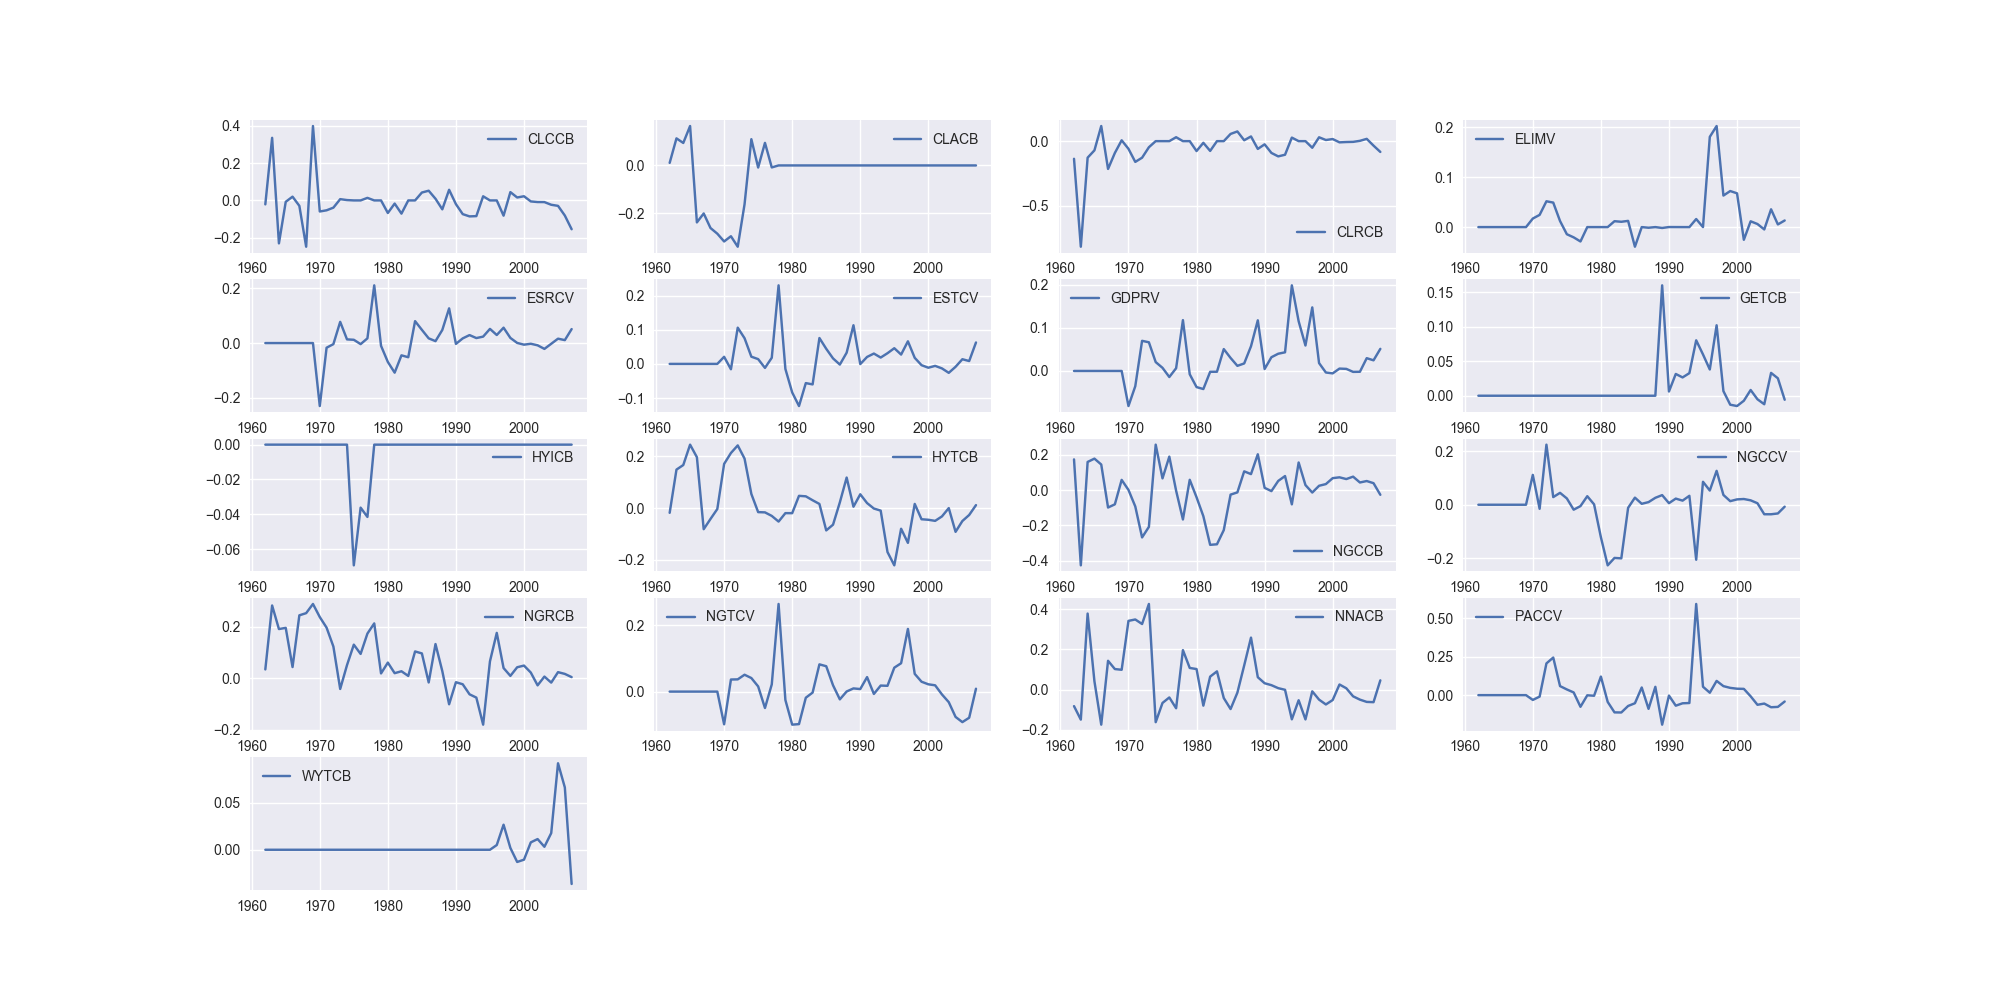
\includegraphics[scale=0.3]{tx.png}
\end{figure}


\begin{thebibliography}{1}	
	\bibitem{}  https://www.sciencedirect.com/science/article/pii/0169743987800849  this is an article change the format to IEEE	
\end{thebibliography}

\end{document}
